\subsection{Diagrammes de s\'{e}quences}
Le diagramme de s\'{e}quence indique l'interaction entre plusieurs acteurs
afin d'expliquer le d\'{e}roulement des diff\'{e}rents sc\'{e}nario entre les diff\'{e}rents
\'{e}l\'{e}ments du projet. Les sch\'{e}mas suivants repr\'{e}sentent dans chaque cas les
diagrammes de s\'{e}quences.
Nous  d\'{e}crivons les sc\'{e}narios les plus importants de notre application qui sont
comme indique dans ce tableau :

\FloatBarrier
\begin{table}[H]
\centering
\begin{tabular}{|l|l|l|}
\hline
                                            & Administrateur & Membre  \\
\hline
Authentification~                           & X              & X       \\
\hline
Création d’un projet                        & X              &         \\
\hline
Ajout d’une tache                           & X              & X       \\
\hline
Modifier l’état d’une tâche                 & X              &         \\
\hline
Ajout d’un client/membre                    & X              &         \\
\hline
Consultation des rapports                   & X              &         \\
\hline
Consulter la carte géographique des clients & X              & X       \\
\hline
\end{tabular}
\end{table}
\FloatBarrier


\newpage

\subsubsection{ Le sc\'{e}nario \guillemotleft{} Authentification \guillemotright{}}
Ce sch\'{e}ma pr\'{e}sente le m\^{e}me sc\'{e}nario pour l'administrateur et un simple
membre:


\begin{figure}[H]
\center
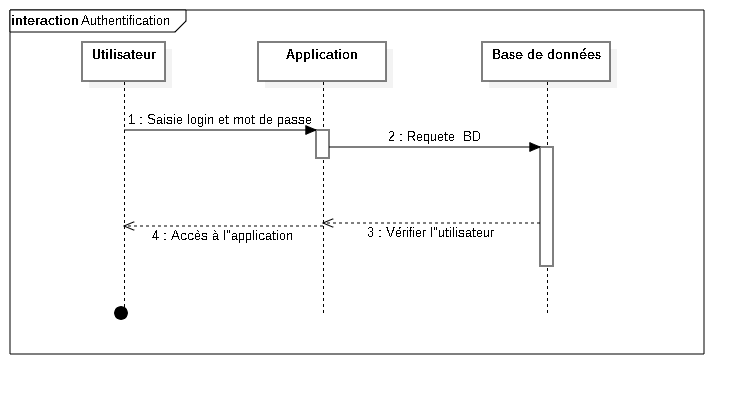
\includegraphics[width=14cm,height=8cm]{./figures/seq/A.png}
\caption{Authentification.}
\end{figure}

\newpage
\subsubsection{  Le sc\'{e}nario \guillemotleft{} Cr\'{e}ation d'un projet \guillemotright{}}

Le diagramme de s\'{e}quence \guillemotleft{} Ajout d'un projet \guillemotright{} pr\'{e}sente un s\'{e}quencement
des interactions entre Administrateur, Application et Base de donn\'{e}es (BD) .


\begin{figure}[H]
\center
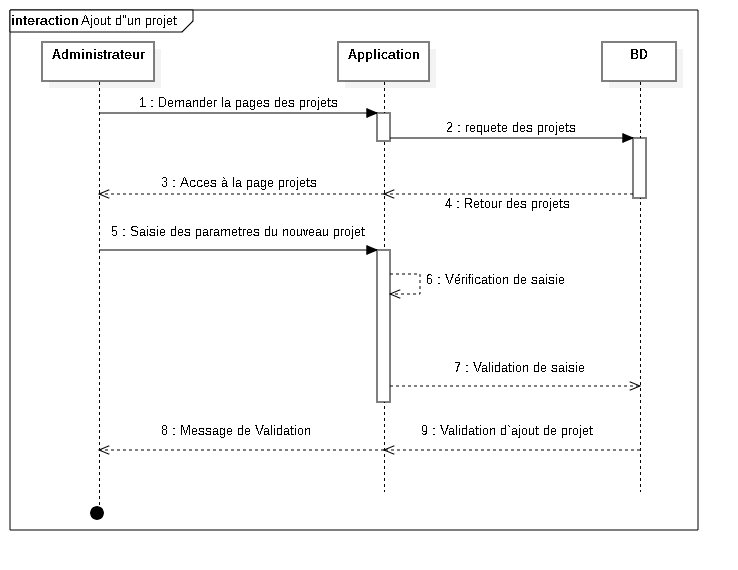
\includegraphics[width=14cm,height=11cm]{./figures/seq/B.png}
\caption{ Cr\'{e}ation d'un projet.}
\end{figure}

\newpage
\subsubsection{Le sc\'{e}nario \guillemotleft{} Cr\'{e}ation d'une t\^{a}che\guillemotright{}}
Le diagramme de s\'{e}quence \guillemotleft{} Ajout d'une t\^{a}che \guillemotright{} pr\'{e}sente le s\'{e}quencement
des interactions entre Administrateur, Application et Base de donn\'{e}es (BD).

\begin{figure}[H]
\center
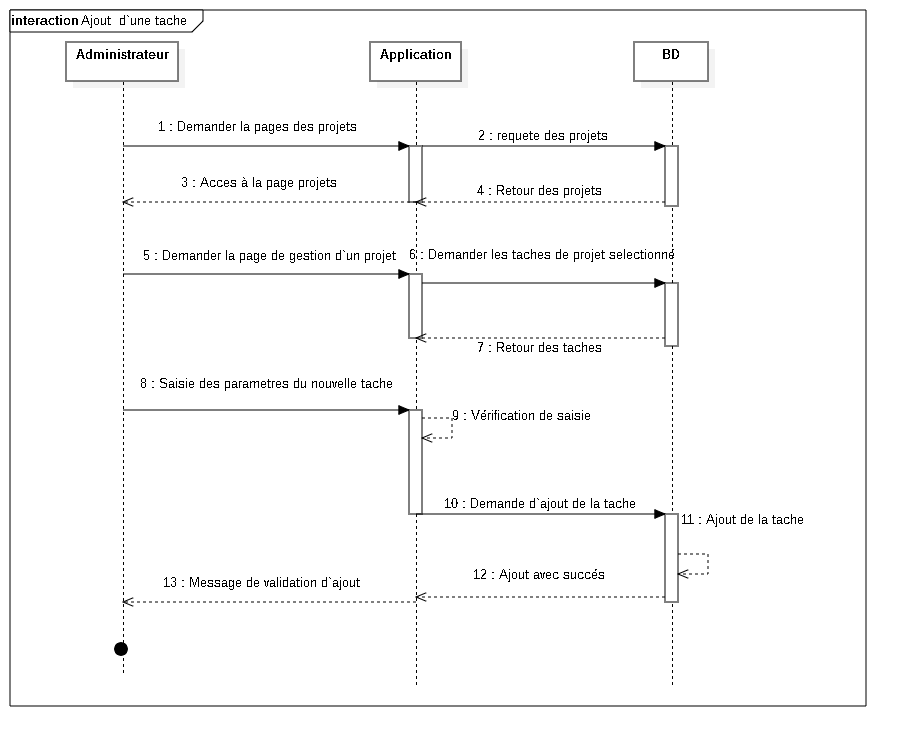
\includegraphics[width=14cm,height=13cm]{./figures/seq/C.png}
\caption{Cr\'{e}ation d'une t\^{a}che.}
\end{figure}


\newpage
\subsubsection{ Le sc\'{e}nario \guillemotleft{} Modification de l`\'{e}tat d'une t\^{a}che\guillemotright{}}

Le diagramme de s\'{e}quence \guillemotleft{} Ajout d'une t\^{a}che \guillemotright{} pr\'{e}sente le s\'{e}quencement
des interactions entre Administrateur, Application et Base de donn\'{e}es (BD).


\begin{figure}[H]
\center
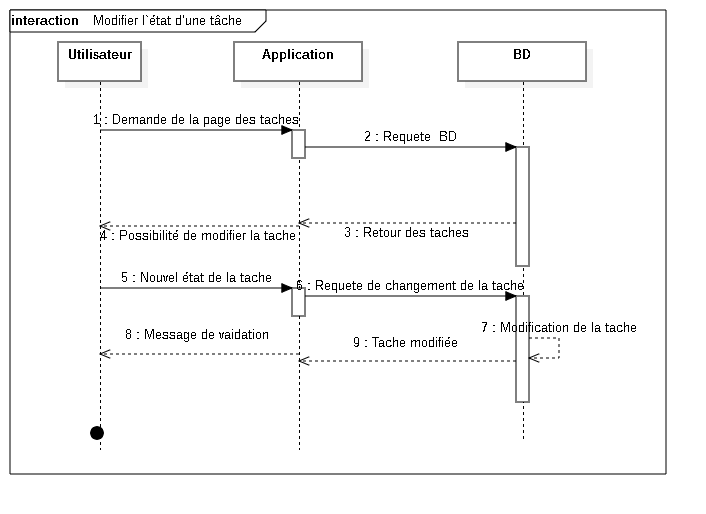
\includegraphics[width=14cm,height=10cm]{./figures/seq/D.png}
\caption{ Modification de l`\'{e}tat d'une t\^{a}che.}
\end{figure}


\newpage
\subsubsection{Le sc\'{e}nario \guillemotleft{} Cr\'{e}ation d'un membre \guillemotright{}}

Le diagramme de s\'{e}quence \guillemotleft{} Ajout d'une t\^{a}che \guillemotright{} pr\'{e}sente le s\'{e}quencement
des interactions entre Administrateur, Application et Base de donn\'{e}es (BD).



\begin{figure}[H]
\center
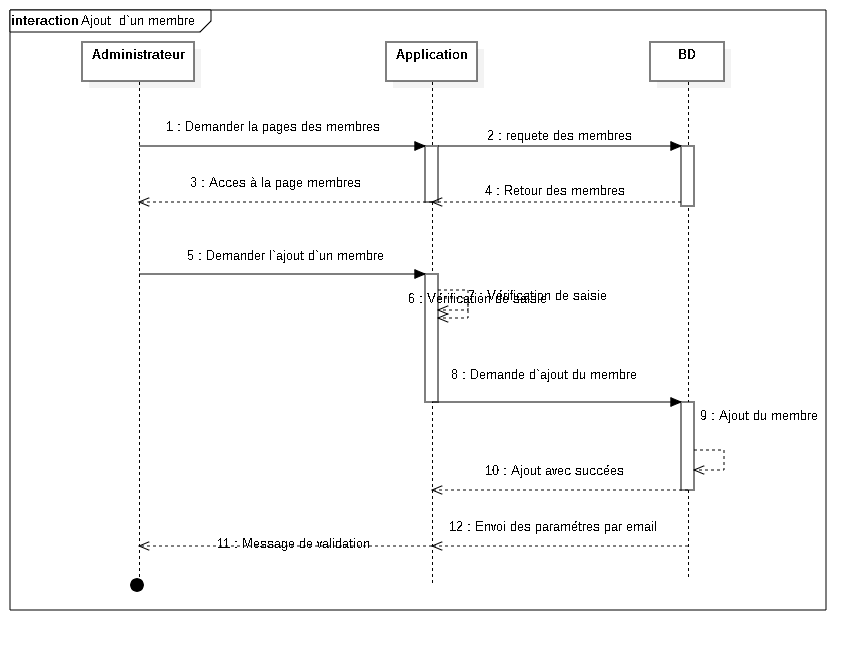
\includegraphics[width=14cm,height=10cm]{./figures/seq/E.png}
\caption{Cr\'{e}ation d'un membre.}
\end{figure}


\subsubsection{Le sc\'{e}nario \guillemotleft{} Cr\'{e}ation d'un client\guillemotright{}}
Le diagramme de s\'{e}quence \guillemotleft{} Ajout d'une t\^{a}che \guillemotright{} pr\'{e}sente le s\'{e}quencement
des interactions entre Administrateur, Application et Base de donn\'{e}es (BD).


\begin{figure}[H]
\center
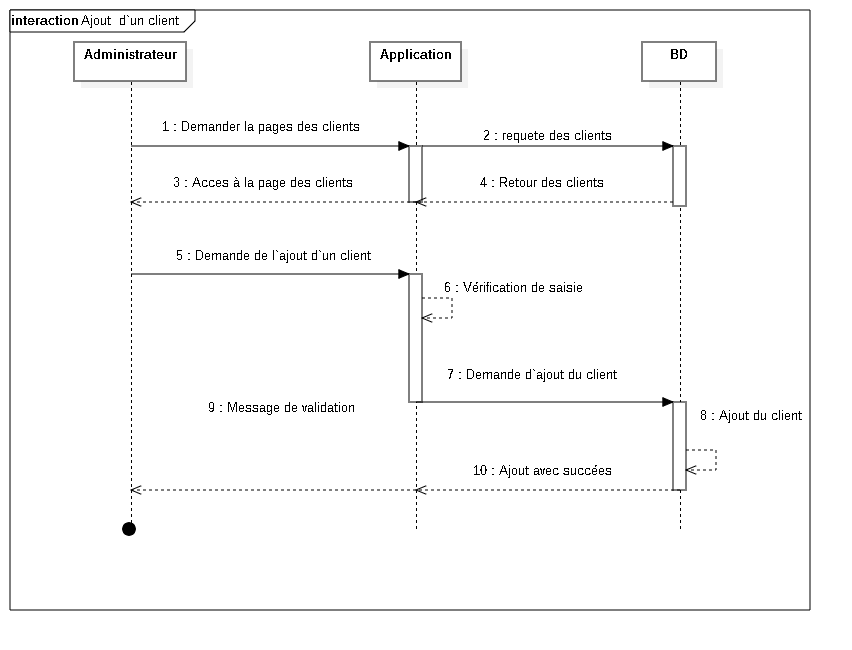
\includegraphics[width=14cm,height=9cm]{./figures/seq/F.png}
\caption{Cr\'{e}ation d'une client.}
\end{figure}

\newpage
\subsubsection{Le sc\'{e}nario \guillemotleft{} Consultation des rapports\guillemotright{}}
Le diagramme de s\'{e}quence \guillemotleft{} Ajout d'une t\^{a}che \guillemotright{} pr\'{e}sente le s\'{e}quencement
des interactions entre Administrateur, Application et Base de donn\'{e}es (BD).


\begin{figure}[H]
\center
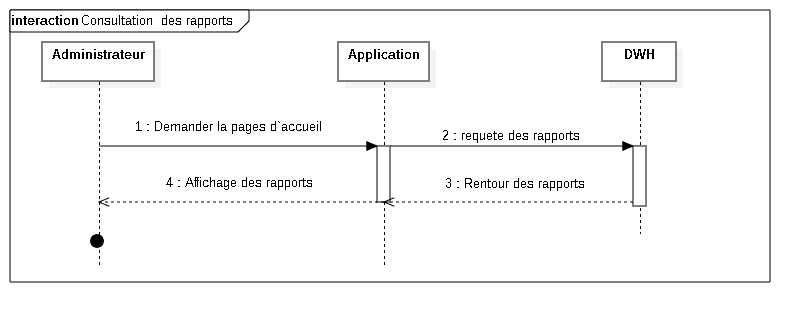
\includegraphics[width=14cm,height=9cm]{./figures/seq/G.png}
\caption{Consultation des rapports.}
\end{figure}


\subsubsection{Le sc\'{e}nario \guillemotleft{} Consultation de la carte g\'{e}ographique des clients\guillemotright{}}
Le diagramme de s\'{e}quence \guillemotleft{} Ajout d'une t\^{a}che \guillemotright{} pr\'{e}sente le s\'{e}quencement
des interactions entre Administrateur, Application et Base de donn\'{e}es (BD).

\begin{figure}[H]
\center
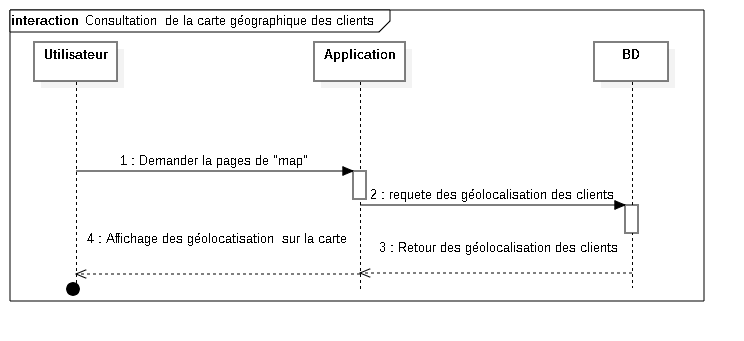
\includegraphics[width=14cm,height=8cm]{./figures/seq/H.png}
\caption{Consultation de la carte g\'{e}ographique des clients.}
\end{figure}
\newpage

